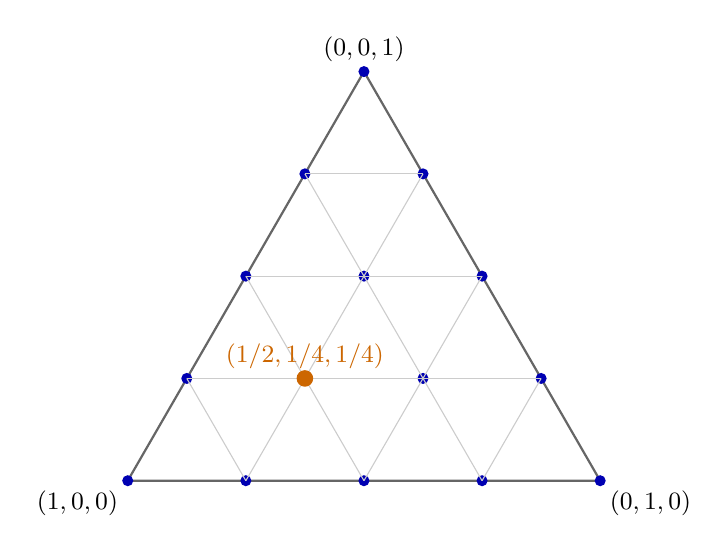
\begin{tikzpicture}[x=1cm,y=1cm]
\draw[black!60,thick] (0,0)--(6,0)--(3,5.196)--cycle;
\foreach \i in {0,1,2,3,4}{
 \foreach \j in {0,1,2,3,4}{
  \ifnum\numexpr\i+\j\relax<5
   \fill[blue!70!black] ({1.5*\i+0.75*\j},{1.299*\j}) circle[radius=2pt];
  \fi
 }
}
\foreach \i in {1,2,3}{
 \draw[black!20] ({1.5*\i},0)--({0.75*\i+3},{5.196-1.299*\i});
 \draw[black!20] ({0.75*\i},{1.299*\i})--({6-0.75*\i},{1.299*\i});
 \draw[black!20] ({1.5*\i},0)--({0.75*\i},{1.299*\i});
}
\fill[orange!80!black] (2.25,1.299) circle[radius=3pt];
\node[above,font=\small,orange!80!black] at (2.25,1.299) {$ (1/2,1/4,1/4)$};
\node[below left,font=\small] at (0,0) {$(1,0,0)$};
\node[below right,font=\small] at (6,0) {$(0,1,0)$};
\node[above,font=\small] at (3,5.196) {$(0,0,1)$};
\end{tikzpicture}
